%%%%%%%%%%%%%%%%%%%%%%%%%%%%%%%%%%%%%%%%% 
% Beamer Presentation
% LaTeX Template
% Version 1.0 (10/11/12)
% 
% This template has been downloaded from:
% http://www.LaTeXTemplates.com
% 
% License:
% CC BY-NC-SA 3.0 (http://creativecommons.org/licenses/by-nc-sa/3.0/)
% 
%%%%%%%%%%%%%%%%%%%%%%%%%%%%%%%%%%%%%%%%% 

% ----------------------------------------------------------------------------------------
%	PACKAGES AND THEMES
% ----------------------------------------------------------------------------------------

\documentclass{beamer}

\mode<presentation> {

  % The Beamer class comes with a number of default slide themes
  % which change the colors and layouts of slides. Below this is a list
  % of all the themes, uncomment each in turn to see what they look like.

  % \usetheme{default}
  % \usetheme{AnnArbor}
  % \usetheme{Antibes}
  % \usetheme{Bergen}
  % \usetheme{Berkeley}
  % \usetheme{Berlin}
  % \usetheme{Boadilla}
  % \usetheme{CambridgeUS}
  % \usetheme{Copenhagen}
  % \usetheme{Darmstadt}
  % \usetheme{Dresden}
  % \usetheme{Frankfurt}
  % \usetheme{Goettingen}
  % \usetheme{Hannover}
  % \usetheme{Ilmenau}
  % \usetheme{JuanLesPins}
  % \usetheme{Luebeck}
  \usetheme{Madrid}
  % \usetheme{Malmoe}
  % \usetheme{Marburg}
  % \usetheme{Montpellier}
  % \usetheme{PaloAlto}
  % \usetheme{Pittsburgh}
  % \usetheme{Rochester}
  % \usetheme{Singapore}
  % \usetheme{Szeged}
  % \usetheme{Warsaw}

  % As well as themes, the Beamer class has a number of color themes
  % for any slide theme. Uncomment each of these in turn to see how it
  % changes the colors of your current slide theme.

  % \usecolortheme{albatross}
  % \usecolortheme{beaver}
  % \usecolortheme{beetle}
  % \usecolortheme{crane}
  % \usecolortheme{dolphin}
  % \usecolortheme{dove}
  % \usecolortheme{fly}
  % \usecolortheme{lily}
  % \usecolortheme{orchid}
  % \usecolortheme{rose}
  % \usecolortheme{seagull}
  % \usecolortheme{seahorse}
  % \usecolortheme{whale}
  % \usecolortheme{wolverine}

  % \setbeamertemplate{footline} % To remove the footer line in all slides uncomment this line
  % \setbeamertemplate{footline}[page number] % To replace the footer line in all slides with a simple slide count uncomment this line

  % \setbeamertemplate{navigation symbols}{} % To remove the navigation symbols from the bottom of all slides uncomment this line
}

\usepackage{graphicx} % Allows including images
\usepackage{multirow}
\usepackage{booktabs} % Allows the use of \toprule, \midrule and \bottomrule in tables
\graphicspath{ {images/} }

% ----------------------------------------------------------------------------------------
%	TITLE PAGE
% ----------------------------------------------------------------------------------------

\title[Speeding up Yourself]{Time and Space Saving Technologies in Compilation and Elaboration} % The short title appears at the bottom of every slide, the full title is only on the title page

\author{Guanyu Yi} % Your name
\institute[SPRD] % Your institution as it will appear on the bottom of every slide, may be shorthand to save space
{
  Spreadtrum Communications, Inc. \\ % Your institution for the title page
  \medskip
  \textit{gary3511@gmail.com} % Your email address
}
\date{August 13, 2015} % Date, can be changed to a custom date

\begin{document}

\begin{frame}
  \titlepage % Print the title page as the first slide
\end{frame}

\begin{frame}
  \frametitle{Overview} % Table of contents slide, comment this block out to remove it
  \tableofcontents % Throughout your presentation, if you choose to use \section{} and \subsection{} commands, these will automatically be printed on this slide as an overview of your presentation
\end{frame}

% ----------------------------------------------------------------------------------------
%	PRESENTATION SLIDES
% ----------------------------------------------------------------------------------------

% ------------------------------------------------
\section{Backgrounds} % Sections can be created in order to organize your presentation into discrete blocks, all sections and subsections are automatically printed in the table of contents as an overview of the talk
% ------------------------------------------------

% \subsection{Subsection Example} % A subsection can be created just before a set of slides with a common theme to further break down your presentation into chunks

\begin{frame}
  \frametitle{Backgrounds}
  \begin{columns}[c] % The "c" option specifies centered vertical alignment while the "t" option is used for top vertical alignment

    \column{.45\textwidth} % Left column and width
    \textbf{Chip size and gate number}
    \begin{enumerate}
    \item Millimeter scale chip size
    \item Billions of transistors
    \end{enumerate}
    \begin{figure}
      \centering
      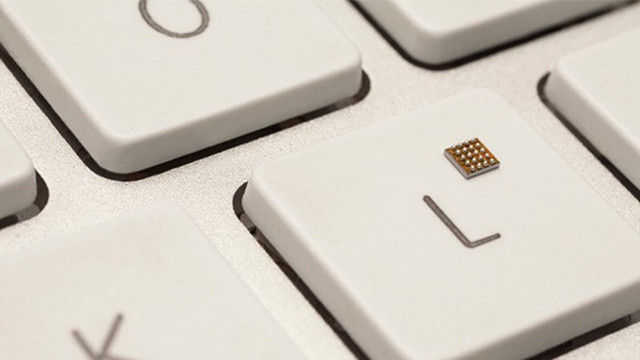
\includegraphics[width=0.9\linewidth]{chip_size}
      \caption{World smallest ARM chip, 1.9mm$\times$2.2mm}
    \end{figure}

    \column{.5\textwidth} % Right column and width
    \begin{figure}
      \centering
      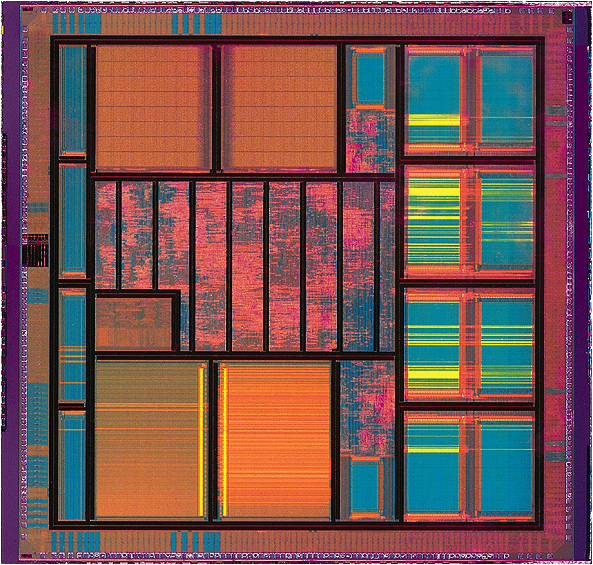
\includegraphics[width=0.9\linewidth]{chip_gates}
      \caption{Intel's 4th generation i7 Extreme silicon with billions of transistors}
    \end{figure}

  \end{columns}
\end{frame}

% ----------------------------------------------------------------------------------------

\begin{frame}
  \frametitle{Backgrounds}
  \begin{block}{Challenges}
    \begin{enumerate}
    \item Huge time and disk space consumption
    \item Regression
    \item Gate level simulation
    \end{enumerate}
  \end{block}

  \begin{table}
    \centering
    \begin{tabular}{lll}
      \toprule
      & \textbf{time consumption}* & \textbf{space consumption} \\
      \midrule
      single case & 23.3min & 5.5G \\
      1000\texttt{+} cases & 16.1day\texttt{+} & 5.5T\texttt{+} \\
      single GL case & 255.3min & 15.0G \\
      100\texttt{+} GL case & 17.7day\texttt{+} & 1.5T\texttt{+} \\
      \bottomrule
      \multicolumn{3}{l}{\footnotesize{* compilation and elaboration time}}
    \end{tabular}
    \caption{Consumption of time and space}
  \end{table}
\end{frame}

% ------------------------------------------------
\section{Compilation and Elaboration}
% ------------------------------------------------

\begin{frame}
  \frametitle{Compilation and Elaboration}
  \begin{columns}[c] % The "c" option specifies centered vertical alignment while the "t" option is used for top vertical alignment

    \column{.45\textwidth} % Left column and width
    \textbf{Main stages}
    \begin{enumerate}
    \item Compiling DUT into libraries
    \item Elaborating libraries into snapshots
    \item Using snapshots for simulation
    \item Integrating compilation and elaboration into common flow
    \end{enumerate}

    \column{.5\textwidth} % Right column and width
    \begin{figure}
      \centering
      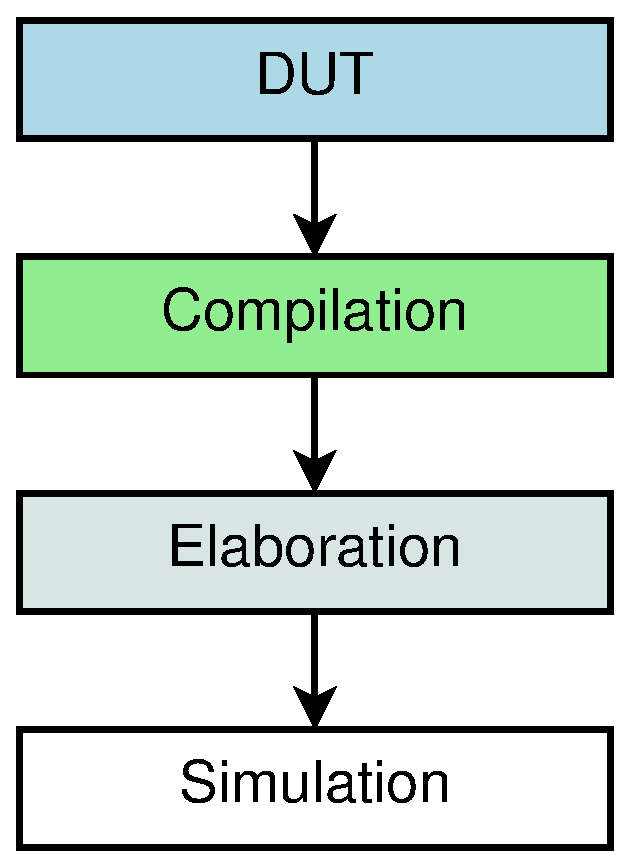
\includegraphics[width=0.6\linewidth]{simulation_stages}
      \caption{Cadence EDA simulation stages}
    \end{figure}

  \end{columns}
\end{frame}

% ------------------------------------------------
\section{Time and Space Saving Technologies}
% ------------------------------------------------

\begin{frame}
  \frametitle{Time and Space Saving Technologies}
  \begin{block}{Parallel technology}
    Parallel computing is a form of computation in which many calculations are carried out simultaneously.
  \end{block}

  \begin{block}{Pre-compilation}
    Pre-compile files into libraries with the \textit{-compile} and \textit{-makelib} options, and then refer to the libraries with the \textit{-reflib} option for elaboration.
  \end{block}

  \begin{block}{MSIE}
    Multi-snapshot incremental elaboration(MSIE) provides a form of incremental elaboration that can greatly decrease the time it takes to re-elaborate a design.
  \end{block}
\end{frame}

% ----------------------------------------------------------------------------------------

\begin{frame}
  \frametitle{Time and Space Saving Technologies}
  \begin{columns}[c] % The "c" option specifies centered vertical alignment while the "t" option is used for top vertical alignment

    \column{.45\textwidth} % Left column and width
    \textbf{Parallel technology}
    \begin{enumerate}
    \item Multi-threading
    \item Multi-processing
    \item Platform Load Sharing Sacility (LSF)
    \end{enumerate}

    \column{.5\textwidth} % Right column and width
    \begin{figure}
      \centering
      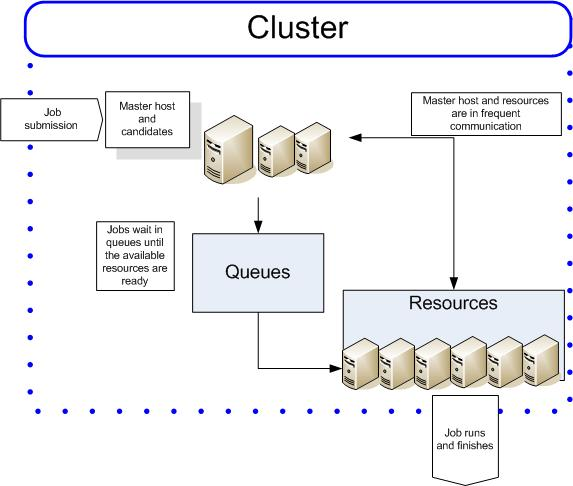
\includegraphics[width=\linewidth]{lsf_cluster_overview}
      \caption{IBM Platform LSF overview}
    \end{figure}

  \end{columns}
\end{frame}

% ----------------------------------------------------------------------------------------

\begin{frame}
  \frametitle{Time and Space Saving Technologies}
  \begin{columns}[c] % The "c" option specifies centered vertical alignment while the "t" option is used for top vertical alignment

    \column{.45\textwidth} % Left column and width
    \textbf{Pre-compilation}
    \begin{enumerate}
    \item IP and std\_cell collection
    \item RTL design splitting
    \item Verilog and VHDL
    \item Various types of each library
    \item Make use of parallel technology
    \item Base of MSIE
    \end{enumerate}

    \column{.5\textwidth} % Right column and width
    \begin{figure}
      \centering
      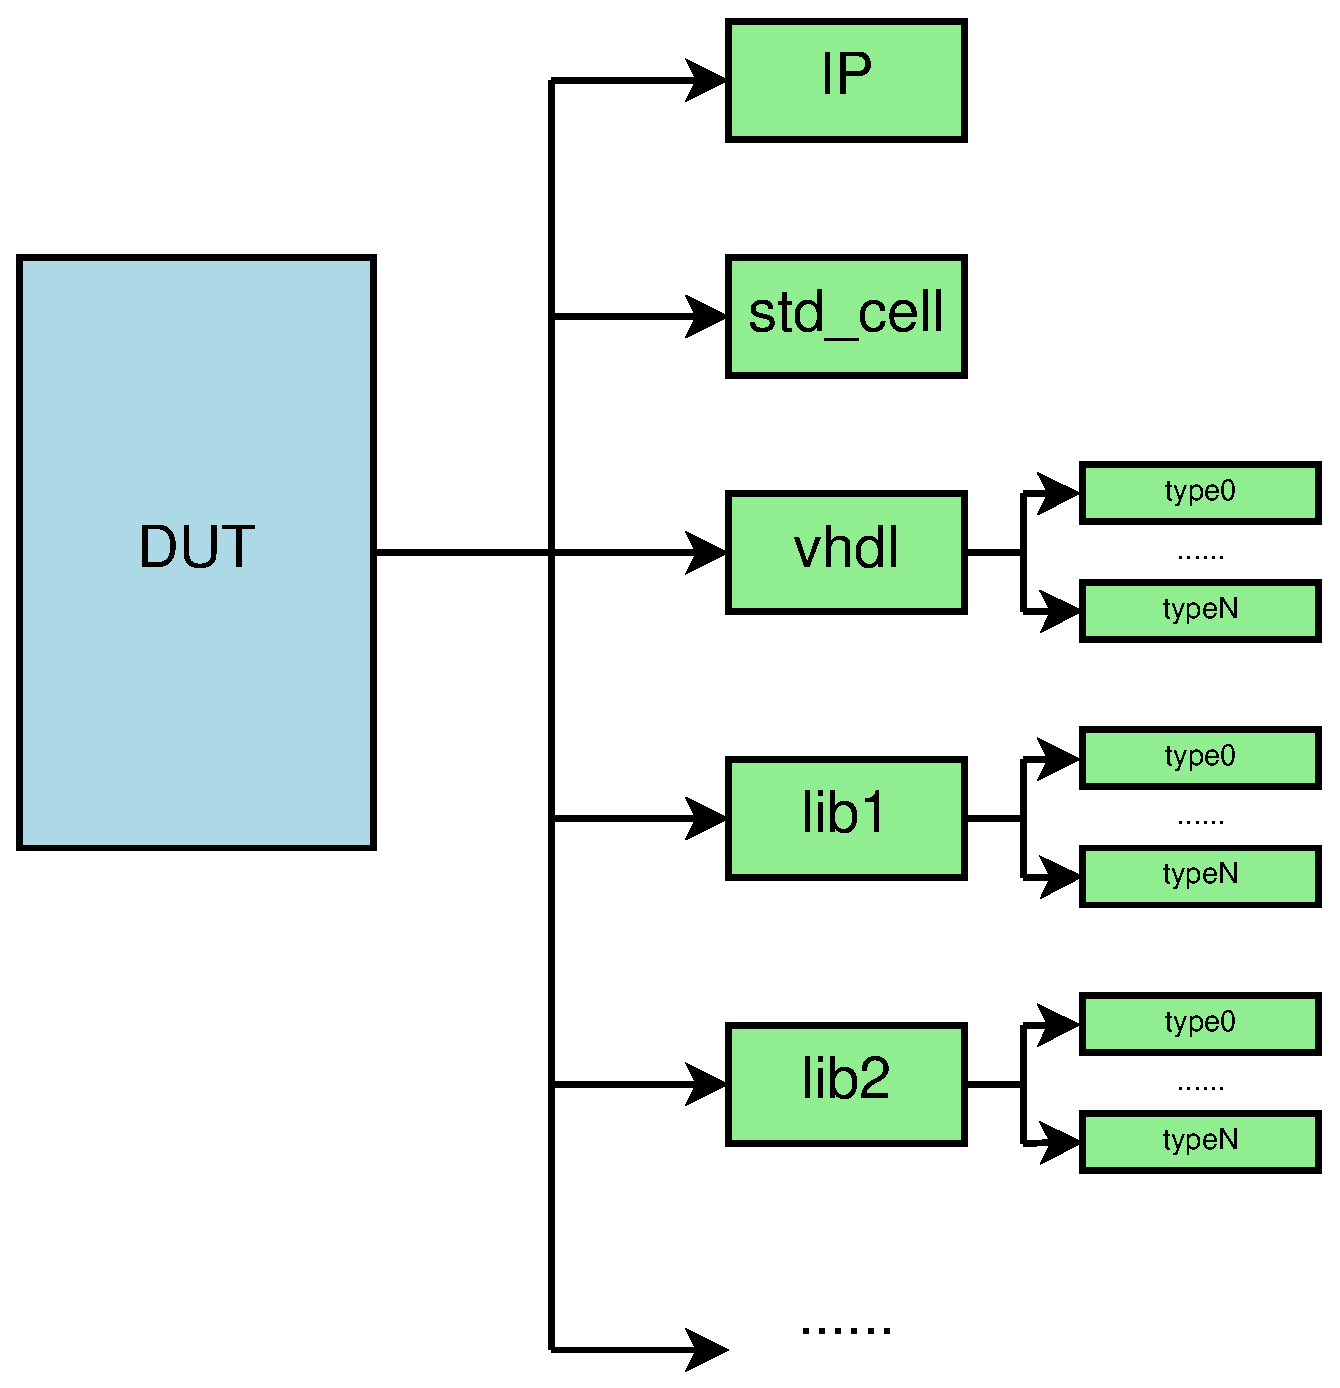
\includegraphics[width=0.9\linewidth]{dut_split}
      \caption{DUT splitting and parallel processing}
    \end{figure}

  \end{columns}
\end{frame}

% ----------------------------------------------------------------------------------------

\begin{frame}
  \frametitle{Time and Space Saving Technologies}
  \begin{columns}[c] % The "c" option specifies centered vertical alignment while the "t" option is used for top vertical alignment

    \column{.45\textwidth} % Left column and width
    \textbf{MSIE}
    \begin{enumerate}
    \item Elaborating from corresponding libraries
    \item Elaborating TB incrementally
    \item Make use of parallel technology
    \item Make use of pre-compilation
    \end{enumerate}

    \column{.5\textwidth} % Right column and width
    \begin{figure}
      \centering
      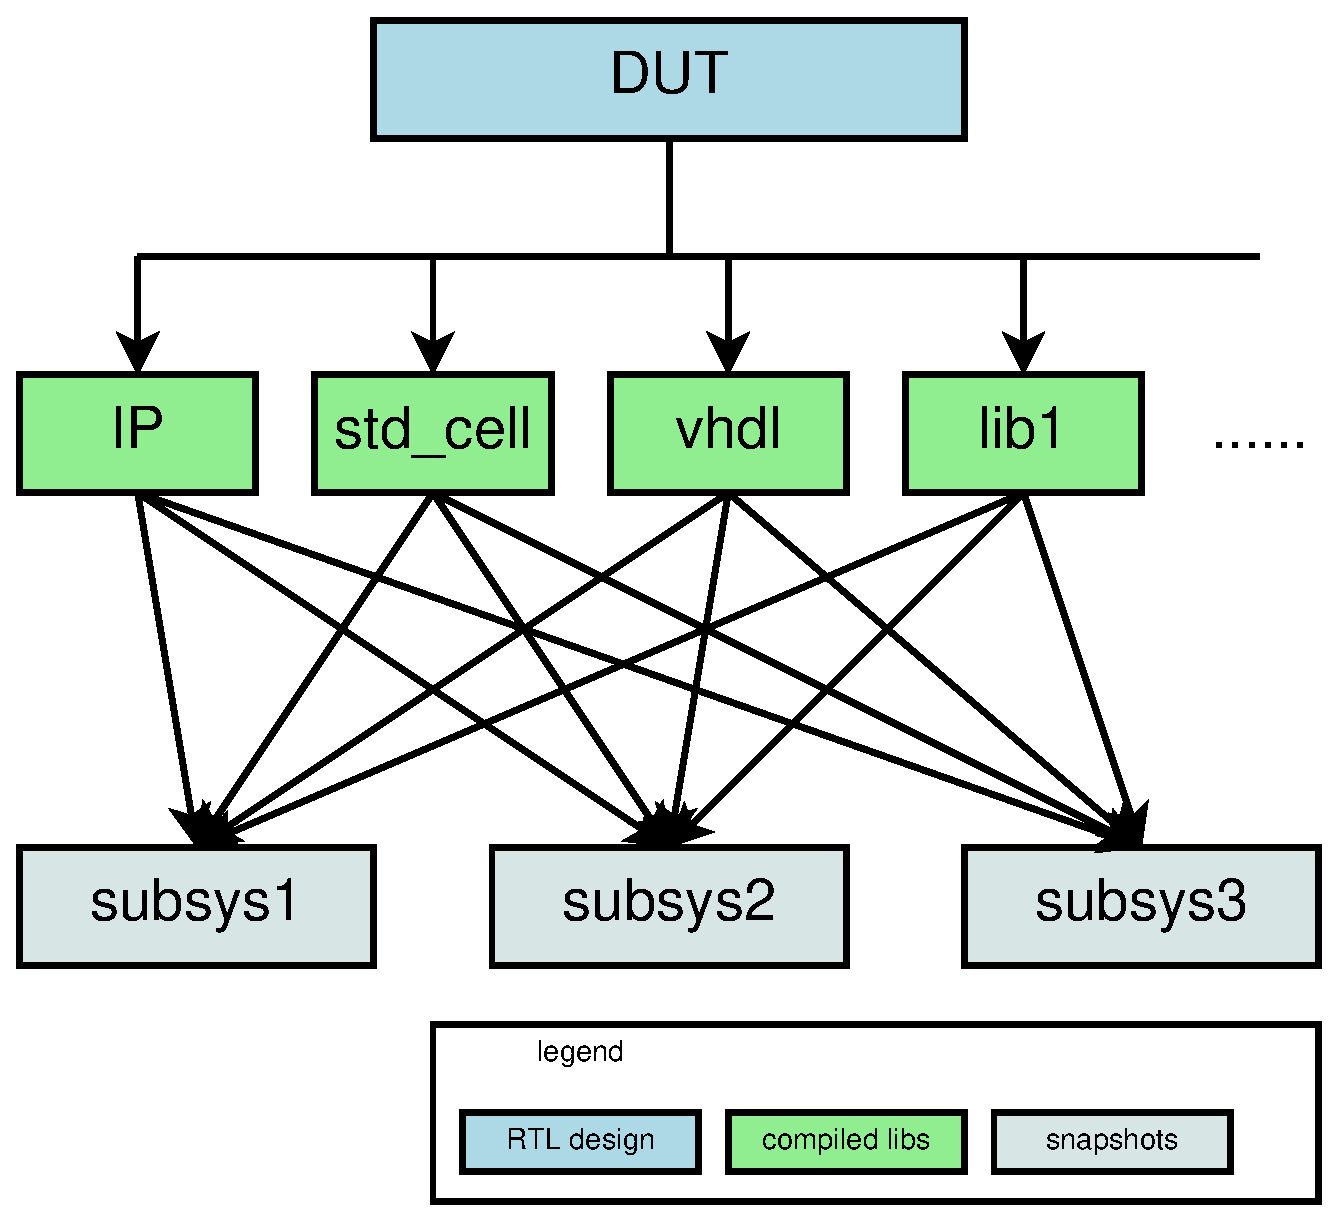
\includegraphics[width=0.9\linewidth]{pm_mapping}
      \caption{Libraries and snapshots mapping}
    \end{figure}

  \end{columns}
\end{frame}

% ----------------------------------------------------------------------------------------

\begin{frame}
  \frametitle{Time and Space Saving Technologies}
  \begin{columns}[c] % The "c" option specifies centered vertical alignment while the "t" option is used for top vertical alignment

    \column{.45\textwidth} % Left column and width
    \textbf{Parallel processing}
    \begin{enumerate}
    \item Multiprocessing module in python
      \begin{enumerate}
      \item pre-processing
      \item container of distribution jobs
      \end{enumerate}
    \item LSF for compilation and elaboration
    \end{enumerate}

    \column{.5\textwidth} % Right column and width
    \begin{figure}
      \centering
      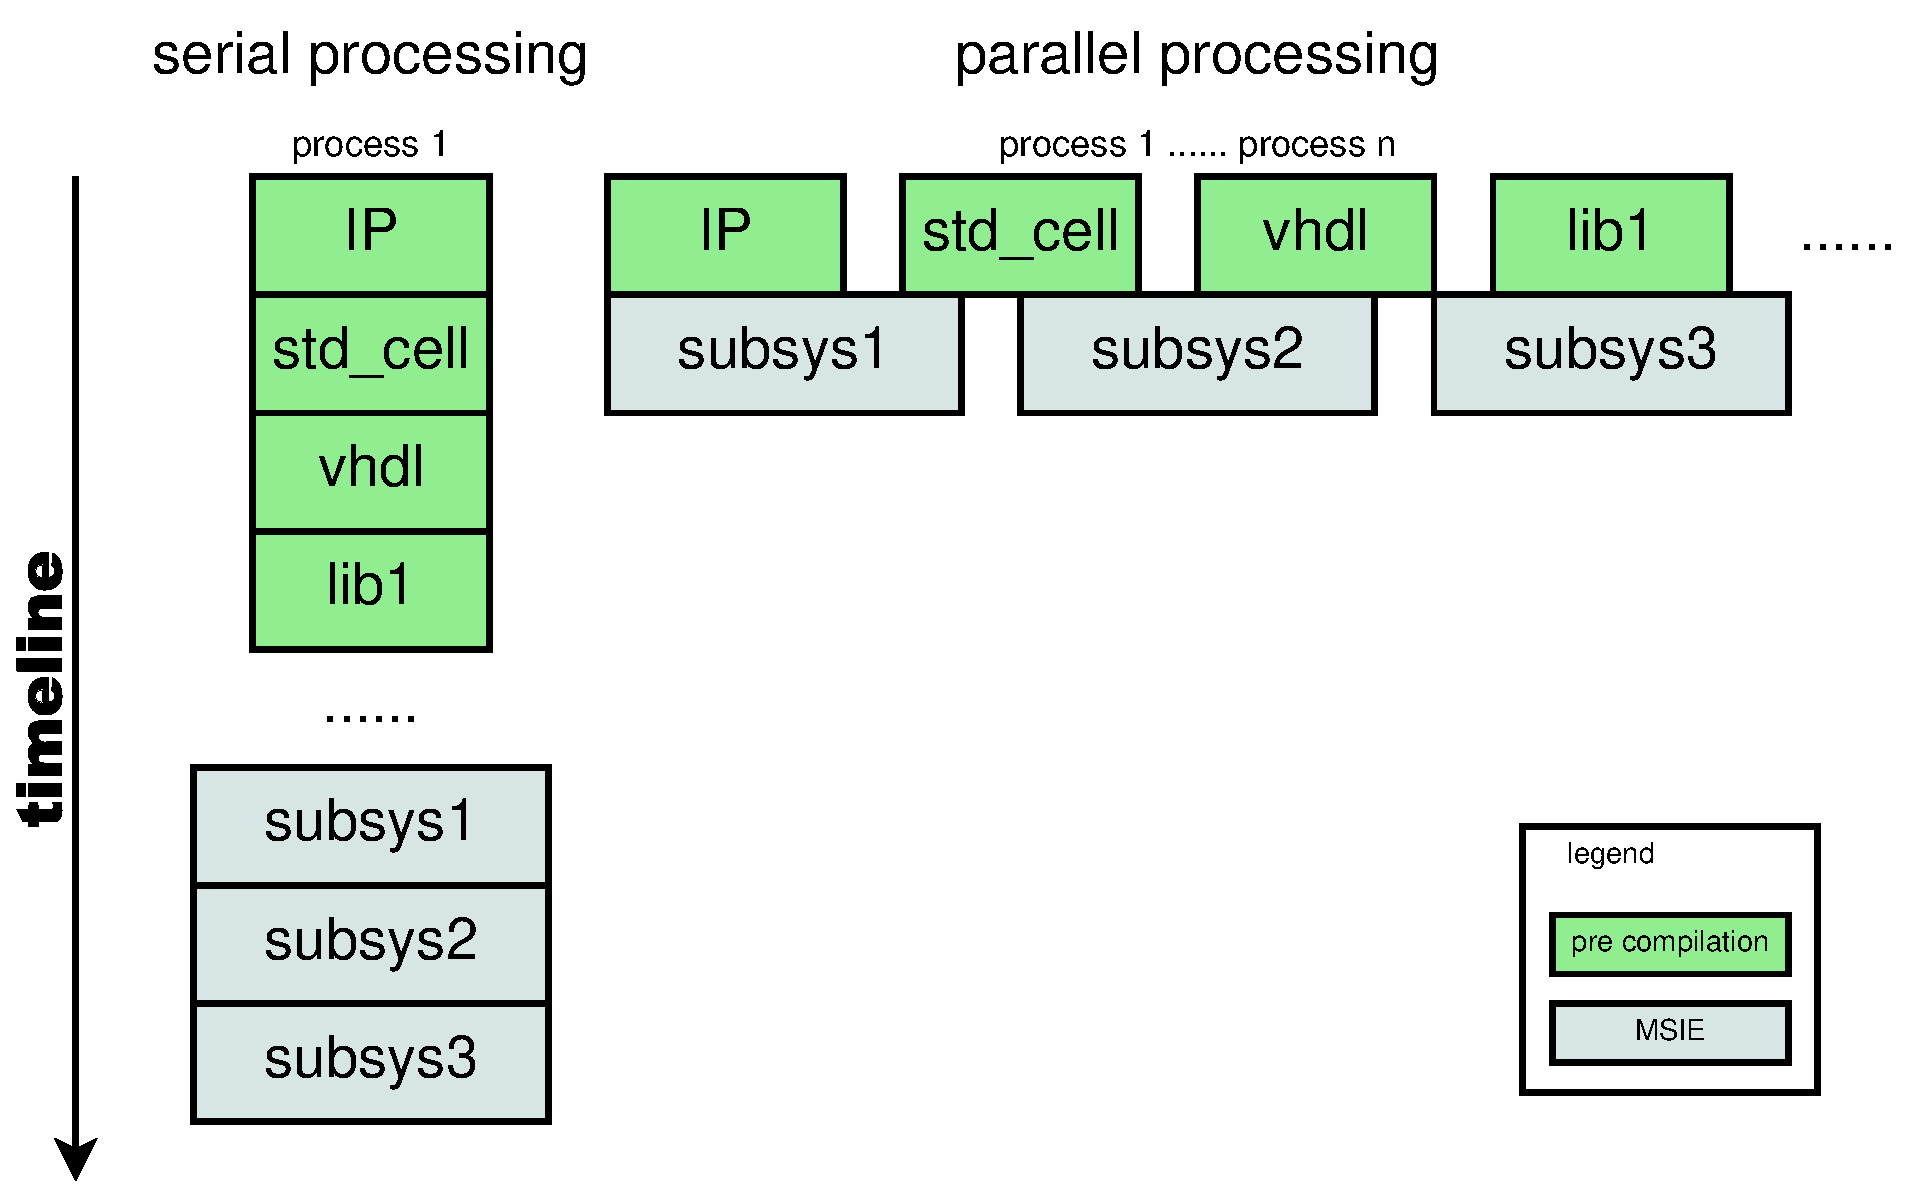
\includegraphics[width=0.9\linewidth]{parallel}
      \caption{Parallel processing overview}
    \end{figure}

  \end{columns}
\end{frame}

% ------------------------------------------------
\section{Experiment and Results}
% ------------------------------------------------

\begin{frame}
  \frametitle{Experiment and Results}
  \textbf{5 steps of implementing MSIE in regression}
  \begin{itemize}
  \item Pre-compilation on split DUT
  \item MSIE elaboration based on libraries
  \item Href files generation, 2 sub steps
    \begin{itemize}
    \item generating separated href file each case
    \item merging all href files together
    \end{itemize}
  \item Snapshot re-elaboration with href files
  \item Incremental elaboration of TB
  \end{itemize}
\end{frame}

% ----------------------------------------------------------------------------------------

\begin{frame}
  \frametitle{Experiment and Results}
  \begin{table}
    \centering
    \begin{tabular}{lllll}
      \toprule
      \textbf{steps} & \textbf{time new} & \textbf{time legacy} &  \textbf{space new} & \textbf{space legacy} \\
      \midrule
      pre comp & 1min 12sec* & \multirow{5}{*}{23min 22sec} & 4.3G* & \multirow{5}{*}{5.5G} \\
      \cline{1-2}\cline{4-4}
      MSIE elab & 2min 23sec* & & \multirow{3}{*}{8.7G*} & \\
      \cline{1-2}
      href gen & 2min 29sec* & & & \\
      \cline{1-2}
      re elab & 2min 29sec* & & & \\
      \cline{1-2}\cline{4-4}
      inc elab & 2min 16sec & & 0.2G & \\
      \hline
      total & 2min 16sec & 23min 22sec & 0.2G & 5.5G \\
      \bottomrule
      \multicolumn{5}{l}{\footnotesize{* the time and space marked with star is shared by every case}}
    \end{tabular}
    \caption{Time and space comparison table}
  \end{table}
\end{frame}

% ----------------------------------------------------------------------------------------

\begin{frame}
  \frametitle{Experiment and Results}
  \begin{table}
    \centering
    \begin{tabular}{lllll}
      \toprule
      \textbf{steps} & \textbf{time new} & \textbf{time legacy} &  \textbf{space new} & \textbf{space legacy} \\
      \midrule
      pre comp & 15min 12sec* & \multirow{3}{*}{255min 22sec} & 4.3G* & \multirow{3}{*}{15.0G} \\
      \cline{1-2}\cline{4-4}
      MSIE elab & 48min 15sec* & & 8.7G* & \\
      \cline{1-2}\cline{4-4}
      inc elab & 58min 33sec & & 8.1G & \\
      \hline
      total & 58min 33sec & 255min 22sec & 8.1G & 15.0G \\
      \bottomrule
      \multicolumn{5}{l}{\footnotesize{* the time and space marked with star is shared by every case}}
    \end{tabular}
    \caption{Time and space comparison table of GLS}
  \end{table}
\end{frame}

% ------------------------------------------------
\section{Implementation Issues}
% ------------------------------------------------

\begin{frame}
  \frametitle{Implementation Issues}
  \textbf{Href files handling}
  \begin{itemize}
  \item 3 out of 5 steps are about href files
  \item Hierarchy permission
  \item Test case based
  \item \textit{-primhrefupdate} option for single case scenario
  \item Flexible concurrent method for regression scenario
  \end{itemize}
\end{frame}

% ----------------------------------------------------------------------------------------

\begin{frame}
  \frametitle{Implementation Issues}
  \textbf{Verilog configuration simplicity}
  \begin{itemize}
  \item Elaboration reference conflict
  \item Not a tool issue but related to RTL design
  \item Verilog configuration to solve conflict
  \item \textit{-libmap} option for simply figuring out reference order
  \end{itemize}
\end{frame}

% ----------------------------------------------------------------------------------------

\begin{frame}
  \Huge{\centerline{Q \& A}}
\end{frame}

% ----------------------------------------------------------------------------------------

\end{document}
%%% Local Variables:
%%% mode: latex
%%% TeX-master: t
%%% End:
